% Williams Physics Thesis template
% Patterned after the work of Cole Meisenhelder '15
% Commented by Prof. Charlie Doret, 12/2016
% Uploaded to Overleaf by Dr. Kevin Flaherty, 5/2021
% Updated for GEOS by Prof. Alice Bradley, 9/2022

\documentclass[12pt, oneside]{book} 

% The \usepackage{} command will import predefined fonts, symbols, environments, etc.  For example, the ams packages below come from the American Mathematical Society and include all kinds of useful math symbols like integrals
\usepackage{amscd}
\usepackage{amsmath}
\usepackage{amssymb}
\usepackage{amsthm}
\usepackage{verbatim}
\usepackage[utf8]{inputenc}
\usepackage{geometry}                		% See geometry.pdf to learn the layout options. There are lots.
\geometry{letterpaper}                   		% ... or a4paper or a5paper or ... 
%\geometry{landscape}                		% Activate for for rotated page geometry
\usepackage[pdftex]{graphicx}				% Use pdf, png, jpg, or eps� with pdflatex; use eps in DVI mode	
\usepackage{setspace}
\usepackage{physics}
\usepackage{subcaption}
\usepackage[authoryear]{natbib}
\usepackage{pdfpages}
\usepackage{siunitx}
\usepackage{fancyhdr}
\usepackage{float}
\usepackage{graphicx}
\usepackage{listings}
\usepackage{bm}
\usepackage{appendix}
\usepackage{url}
\usepackage{longtable}
\usepackage{setspace}
\usepackage{booktabs}
\usepackage{multirow} % For multirow in tables
\usepackage{wrapfig}% enables the use of \wrapfig, for figures with text wrapped around them
%\usepackage{lipsum}% gives access to \lipsum, which dumps some latin text into your document as filler if you want to check formatting

%\usepackage[parfill]{parskip}    		% Activate to begin paragraphs with an empty line rather than an indent

% Here we set the page dimensions to match the standard thesis format.  These values should not be changed.
%%% SET LENTGH AND WIDTH %%%
\setlength{\textwidth}{6.5in}
\setlength{\textheight}{8.5in}
\setlength{\oddsidemargin}{0pt}
\setlength{\evensidemargin}{0pt}
\setlength{\topmargin}{0pt}
\setlength{\marginparsep}{0pt}
\setlength{\marginparwidth}{1in}

%\begin{document} starts LaTeX looking for actual content.  Everything above this point is purely formatting.
\begin{document}

\begin{titlepage}
\begin{center}

% \vspace* creates some vertical white space on the page to make the title page look more pleasing.  \vspace would do much the same thing, but would not insert the white space if we were at the top of a fresh page.  As this is the start of the document we're obviously at the beginning of a page, so the asterisk is necessary to ensure we still put in two cm of white space.
\vspace*{2cm}

{\huge Change the title} % \huge sets the font size.  Other options include things like \large, \Large, \small, \tiny, etc.

\vspace{2cm}

{\large by\\And Author}

\vspace{2cm}
{Professor Alice Bradley, Advisor}

% \vfill creates an arbitrary amount of vertical white space as necessary to fill the page
\vfill

A thesis submitted in partial fulfillment\\
of the requirements for the\\
Degree of Bachelor of Arts with Honors\\
in Geoscience

\vspace*{3cm}

WILLIAMS COLLEGE\\
Williamstown, Massachusetts\\
\today % you might choose to set a permanent date, but \today will put in today's date
\end{center}
\end{titlepage}


% \frontmatter defines the pieces of the thesis which will use roman numerals for page numbering
\frontmatter 


\onehalfspacing

\chapter{Abstract}
Roughly 200 words for an abstract

\chapter{Acknowledgments}
Say nice things to people here. 


% Table of contents, figure list, and table list
\tableofcontents
\listoffigures
\listoftables

% \mainmatter defines the main body of the thesis and marks where regular numbering will begin
\mainmatter

\chapter{Introduction}
 
Lorem ipsum dolor sit amet, consectetur adipiscing elit. Curabitur non tempor tellus, et placerat orci. Suspendisse dictum leo sed elementum tincidunt. Suspendisse lacinia nunc non ligula vestibulum suscipit. Sed vel nisi id erat ultricies fermentum et ut lorem. Donec sodales magna et efficitur gravida. Maecenas eget porttitor mi. Aliquam tincidunt dignissim ante, sed fringilla lectus ornare id.

Suspendisse egestas, velit viverra porttitor aliquet, lectus ligula sollicitudin risus, sit amet interdum odio velit non neque. Suspendisse quis lectus at arcu sodales mollis eget non justo. Aenean tristique efficitur eleifend. Ut eu faucibus quam. Aliquam ac est rhoncus elit vulputate dignissim eget eget erat. Vestibulum luctus quis magna a molestie. Donec ullamcorper ante ac lectus ultrices bibendum. 



Sed porta volutpat ipsum at finibus. Duis a pulvinar enim. Quisque et risus at dolor lobortis finibus at vitae enim. Curabitur porttitor purus vel arcu placerat, sed ullamcorper leo molestie. Proin dui metus, laoreet nec tempus eu, dictum ut mauris. Sed vitae velit a augue malesuada mattis eget id magna. Cras tincidunt lorem vel sem egestas, eget interdum mauris pharetra. Quisque placerat nulla id erat vulputate, ut scelerisque dui cursus. Nulla rhoncus fringilla arcu eu lobortis. Etiam vulputate elit sed dolor efficitur volutpat.


\begin{figure}
    \centering
    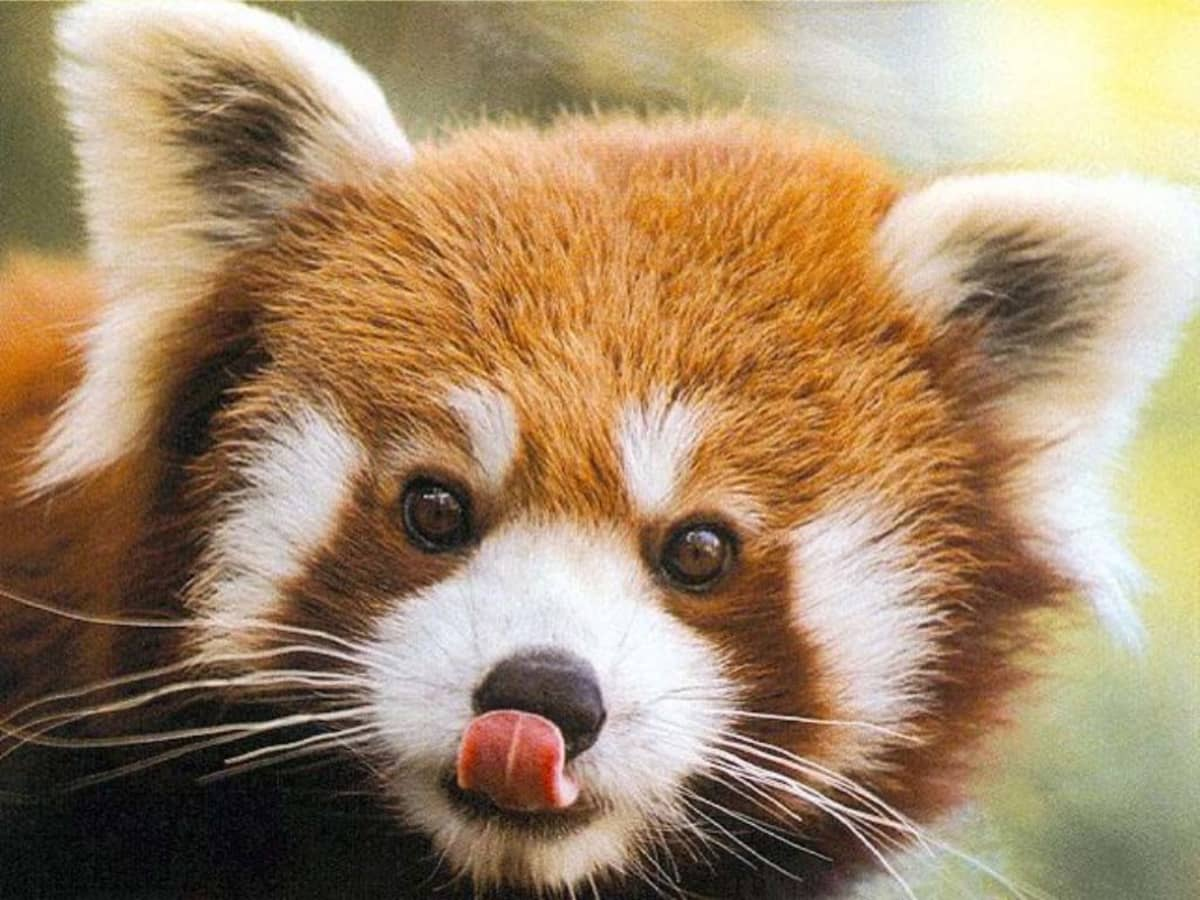
\includegraphics[width=0.5\linewidth]{Chapters//Figures/DifferentFigure.jpg}
    \caption{This is where you write a figure caption. }
    \label{fig:panda}
\end{figure}
Aenean non sapien a purus tincidunt accumsan sit amet eget lacus (see Figure \ref{fig:panda}. Donec hendrerit mauris et tincidunt egestas. Sed interdum, urna eget mattis consequat, dolor justo condimentum enim, non porta nisl felis eget dolor. Aliquam non felis eget ligula suscipit gravida. Sed aliquam blandit neque in bibendum. Vestibulum fringilla neque mauris. Nunc scelerisque libero mauris, non laoreet diam faucibus vel. Integer quis risus sed lectus maximus auctor convallis sit amet massa. Nullam scelerisque faucibus elit. Nulla felis sapien, sagittis ut congue eu, dapibus id augue.

Vestibulum bibendum in lorem sed malesuada. Praesent at volutpat est. Duis dapibus erat in sem egestas ullamcorper. Nulla malesuada felis a est placerat maximus. Vivamus ultricies aliquam consequat. Quisque blandit pulvinar neque, ac vulputate arcu accumsan vitae. Nunc porta justo eu tortor faucibus, eu commodo magna dapibus. Vivamus at iaculis orci. Praesent interdum sem quis ante pulvinar vehicula. Nunc ac mauris nec enim molestie varius. Mauris hendrerit sapien at est tempus, at tempor purus lacinia.

\chapter{Data}
Definitely need this chapter if you're using any data from any sources. 

\section{This is how you do sections}

\subsection{And this is a subsection}



\begin{wrapfigure}{R}{0.6\textwidth}
    \begin{center}
    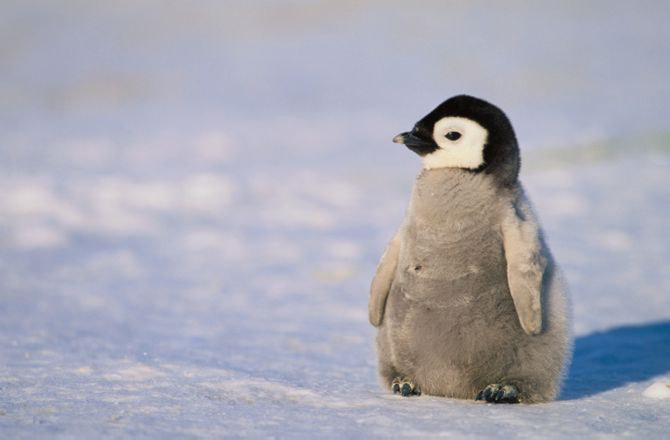
\includegraphics[width=\textwidth]{Chapters/Figures/FigureExample.jpeg}
    \caption{This is a figure caption. That is a penguin.}
    \end{center}
    \label{fig:penguin}
\end{wrapfigure}


Then you can refer to a figure in the text, like Figure \ref{fig:penguin}. 

\begin{table}[H]
    \centering
    \begin{tabular}{ccccccc}  
    \toprule
         Location & Track & Cycle & Seg & Laser&  Dates & Year\\ 
    \midrule
         Chukchi& 0381 & 14/15 & 05 & GT3L &    16 Jan/17 April& 2022 \\  
         Chukchi& 0373 & 14/15 & 03 & GT2L &  15 Jan/16 April& 2022 \\  
         Chukchi& 0373 & 14/15 & 03 & GT3L & 15 Jan/16 April& 2022 \\  
         Chukchi& 0815 & 14/15 & 03 & GT1L & 13 Feb/15 May& 2022 \\ 
         Chukchi& 0815 & 14/15 & 03 & GT2L & 13 Feb/15 May& 2022 \\  
         Beaufort& 0381 & 14/15 & 05 & GT1L & 16 Jan/17 April& 2022 \\ 
         Beaufort & 0320 & 14/15 & 05 & GT3L & 12 Jan/13 April & 2022 \\
    \bottomrule
    \end{tabular}
    \caption{This is what tables look like}
    \label{tab:icesattracks}
\end{table}


\chapter{Conclusions}
\input{Chapters/Conclusions}

\chapter{Future Work}
This is a section that is mostly helpful as a place to put the ideas you don't have time to pursue. 


\chapter{How to write things in LaTeX}
\section{Welcome to the World of LaTeX}

LaTeX is a powerful typesetting system widely used in academia, particularly in fields like mathematics, computer science, and engineering. Unlike word processors that focus on WYSIWYG (What You See Is What You Get), LaTeX operates on a WYSIWYM (What You See Is What You Mean) principle. You write the content and structure of your document, and LaTeX handles the formatting, resulting in beautifully typeset documents.

\subsection{Basic Structure}

A LaTeX document typically begins with a preamble, where you define the document class and load packages. The main content follows within the \texttt{document} environment.

\begin{verbatim}
\documentclass{article}
\usepackage{amsmath} % Example package

\begin{document}

% Your content here

\end{document}
\end{verbatim}

\begin{itemize}
    \item \texttt{\textbackslash documentclass\{article\}}: Specifies the document type (e.g., article, report, book).
    \item \texttt{\textbackslash usepackage\{amsmath\}}: Loads the \texttt{amsmath} package for advanced mathematical typesetting.
    \item \texttt{\textbackslash begin\{document\}} and \texttt{\textbackslash end\{document\}}: Enclose the main content of your document.
\end{itemize}

Your thesis is written as a book. Also, we've set up the preamble so unless you want to do something weird, you don't need to worry about it. 


\subsection{Text and Paragraphs}

To write text, simply type it. LaTeX automatically handles line breaks and paragraph formatting. A blank line creates a new paragraph.

\begin{verbatim}
This is the first paragraph.

This is the second paragraph.
\end{verbatim}

This is the first paragraph.

This is the second paragraph.


\subsection{Sections and Subsections}

Organizing your document is crucial. LaTeX provides commands for creating sections, subsections, and subsubsections.

\begin{verbatim}
\section{Introduction}
\subsection{Background}
\subsubsection{Previous Work}
Note: a * between the section keyword and the bracket makes it not numbered. 
\subsubsection*{Future Work}
\end{verbatim}

\section{Introduction}
\subsection{Background}
\subsubsection{Previous Work}
\subsubsection*{Future Work}


\subsection{References}
To cite a paper, you will need the reference information to be in the .bib file (bibliography.bib here) and then you do this: 
\begin{verbatim}
    \citep{louis2018testing}. If you want to cite more than one, use \citep{louis2018testing, mcnoleg1996integration}. You can also do an in-text citation with \citet{louis2018testing}. 
\end{verbatim}

That looks like this: 
\citep{louis2018testing}. If you want to cite more than one, use \citep{louis2018testing, mcnoleg1996integration}. You can also do an in-text citation with \citet{louis2018testing}. 

\subsection{Mathematics}

LaTeX excels at typesetting mathematical equations. Inline math is enclosed in single dollar signs (\texttt{\$...\$}), while displayed equations are enclosed in double dollar signs (\texttt{\$\$...\$\$}) or the \texttt{equation} environment.

\begin{verbatim}
The Pythagorean theorem is $a^2 + b^2 = c^2$.

\begin{equation}
    E = mc^2
\end{equation}
\end{verbatim}

which looks like this:
The Pythagorean theorem is $a^2 + b^2 = c^2$.

\begin{equation}
    E = mc^2
\end{equation}

\subsection{Lists}

LaTeX offers environments for creating bulleted and numbered lists.

\begin{itemize}
    \item \texttt{itemize} for bulleted lists.
    \item \texttt{enumerate} for numbered lists.
\end{itemize}

\begin{verbatim}
\begin{itemize}
    \item Item 1
    \item Item 2
\end{itemize}

\begin{enumerate}
    \item First item
    \item Second item
\end{enumerate}
\end{verbatim}

\subsection{Including Images}

To include images, use the \texttt{graphicx} package and the \texttt{includegraphics} command.

\begin{figure}[htbp]
    \centering
    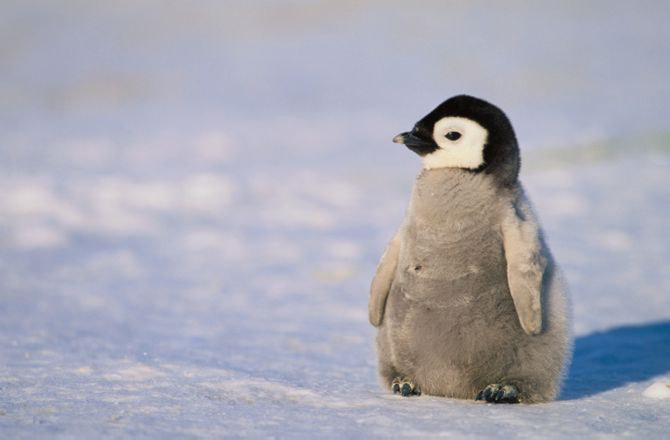
\includegraphics[width=0.5\textwidth]{Chapters/Figures/FigureExample.jpeg}
    \caption{A sample figure caption.}
    \label{fig:sample}
\end{figure}


\begin{verbatim}
\usepackage{graphicx} % Already added to preamble

\begin{figure}[htbp]
    \centering
    \includegraphics[width=0.5\textwidth]{image.png}
    \caption{A sample image.}
    \label{fig:sample}
\end{figure}
\end{verbatim}



\subsection{Tables}

The \texttt{tabular} environment is used to create tables. Note there are tools on the internet that can convert an excel formatted table to a latex one. 

\begin{verbatim}
\begin{tabular}{|c|c|c|}
    \hline
    Header 1 & Header 2 & Header 3 \\
    \hline
    Data 1 & Data 2 & Data 3 \\
    \hline
\end{tabular}
\end{verbatim}

\begin{tabular}{|c|c|c|}
    \hline
    Header 1 & Header 2 & Header 3 \\
    \hline
    Data 1 & Data 2 & Data 3 \\
    \hline
\end{tabular}





Happy typesetting!


% This is the bibliography apsrev, plain
\bibliographystyle{plainnat}
\bibliography{bibliography}

% Here the appendix begins
\appendix 
\chapter{Seasonal Ice Records}
\label{sec:appendix_a}

\section{An Appendix}

This is where you put information and data that isn't core to your explanation, but that you want to not lose. 

Also this is what a table looks like: 


\begin{table}
    \centering
    \begin{tabular}{|l|l|l|}
    \hline
        \textbf{Date} & \textbf{Location} & \textbf{Recorded Ice Behavior} \\ \hline
        2022-06-30 & Utqiaġvik (Barrow) & Pack ice near shore \\ \hline
        2022-06-29 & Utqiaġvik (Barrow) & Break-out of shorefast ice \\ \hline
        2022-06-29 & Utqiaġvik (Barrow) & Pieces of shorefast ice breaking off/Some shorefast ice remaining\\ \hline
        2022-06-27 & Utqiaġvik (Barrow) & Breakup of shorefast ice \\ \hline
        2022-06-27 & Utqiaġvik (Barrow) & Pack ice visible from shore, Some shorefast ice remaining\\ \hline
        2022-06-24 & Utqiaġvik (Barrow) & Shorefast ice is deteriorating \\ \hline
        2022-06-21 & Utqiaġvik (Barrow) & Breakup of shorefast ice \\ \hline
        2022-06-20 & Utqiaġvik (Barrow) & Break-out of shorefast ice \\ \hline
        2022-06-17 & Utqiaġvik (Barrow) & Pack ice near shore \\ \hline
        2022-06-16 & Utqiaġvik (Barrow) & Pieces of shorefast ice breaking off \\ \hline
        2022-06-15 & Utqiaġvik (Barrow) & Pieces of shorefast ice breaking off \\ \hline
        2022-06-14 & Utqiaġvik (Barrow) & Shorefast ice is deteriorating \\ \hline
        2022-06-12 & Utqiaġvik (Barrow) & Pack ice adding to shorefast ice \\ \hline
        2022-06-10 & Utqiaġvik (Barrow) & Pack ice near shore \\ \hline
        2022-05-31 & Utqiaġvik (Barrow) & Lead open \\ \hline
        2022-05-17 & Utqiaġvik (Barrow) & Lead open \\ \hline
        2022-05-16 & Utqiaġvik (Barrow) & Pack ice all packed in \\ \hline
        2022-05-14 & Utqiaġvik (Barrow) & Pack ice all packed in \\ \hline
        2022-05-12 & Utqiaġvik (Barrow) & Pack ice all packed in \\ \hline
        2022-05-11 & Utqiaġvik (Barrow) & Pack ice is moving \\ \hline
        2022-04-19 & Utqiaġvik (Barrow) & Lead open \\ \hline
        2022-04-02 & Utqiaġvik (Barrow) & Lead open \\ \hline
        2022-02-20 & Gravel Pit & Lead open \\ \hline
        2022-01-24 & Gravel Pit & Lead open \\ \hline
        2022-01-18 & Gravel Pit & First stable ice for travel \\ \hline
        2021-12-15 & Piqniq (Duck Camp) & "Ice ridge/s, Shorefast ice is grounded" \\ \hline
        2021-12-13 & Piqniq (Duck Camp) & Shorefast ice is rough \\ \hline
        2021-11-30 & Utqiaġvik (Barrow) & Ice ridge/s, Shorefast ice is thickening\\ \hline
        2021-11-18 & Niksiuraq & Young ice freezing in place \\ \hline
        2021-11-15 & Piqniq (Duck Camp) & Stationary ice along shore \\ \hline
        2021-10-22 & Utqiaġvik (Barrow) & Start freeze up on ocean \\ \hline
    \end{tabular}
    \caption{A summary of observations from the Alaska Arctic Observatory and Knowledge Hub from the 2021-2022 winter season}
\end{table}








\end{document}